\section{Numerical methods}
\label{sec: numerics}

In this section, different techniques will be presented to solve modal and non-modal stability problems for very large-scale dynamical systems. Such very large-scale systems typically arise from the spatial discretization of partial differential equations, e.g.\ the Navier-Stokes equations in fluid dynamics. Throughout this section, the two-dimensional shear-driven cavity flow at various Reynolds numbers will serve as an example. The same configuration as \cite{jfm:sipp:2007} is considered. The dynamics of the flow are governed by
\begin{equation}
  \begin{aligned}
    \displaystyle \frac{\partial \mathbf{U}}{\partial t} + \left( \mathbf{U} \cdot \nabla \right) \mathbf{U} & = - \nabla P + \frac{1}{Re} \nabla^2 \mathbf{U} \\
    \nabla \cdot \mathbf{U} & = 0,
  \end{aligned}
  \label{eq: numerics -- Navier-Stokes equations}
\end{equation}
where $\mathbf{U}$ is the velocity field and $P$ is the pressure field. Figure \ref{fig: numerics -- shear-driven cavity flow} depicts a typical vorticity snapshot obtained from direct numerical simulation at a supercritical Reynolds number.

Given a fixed point $\mathbf{U}_b$ of the Navier-Stokes equations \eqref{eq: numerics -- Navier-Stokes equations}, the dynamics of an infinitesimal perturbation $\mathbf{u}$ evolving on top of it are governed by
\begin{equation}
  \begin{aligned}
    \displaystyle \frac{\partial \mathbf{u}}{\partial t} + \left( \mathbf{u} \cdot \nabla \right) \mathbf{U}_b  + \left( \mathbf{U}_b \cdot \nabla \right) \mathbf{u} & = - \nabla p + \frac{1}{Re} \nabla^2 \mathbf{u} \\
    \nabla \cdot \mathbf{u} & = 0.
  \end{aligned}
  \label{eq: numerics -- linearized Navier-Stokes equations}
\end{equation}
Once projected onto a divergence-free vector space, Eq. \eqref{eq: numerics -- linearized Navier-Stokes equations} can be formally written as
\begin{equation}
  \dot{\mathbf{u}} = \mathbfcal{A}\mathbf{u},
  \label{eq: numerics -- linearized Navier-Stokes equations bis}
\end{equation}
where $\mathbfcal{A}$ is the linearized Navier-Stokes operator. After being discretized in space, $\mathbfcal{A}$ is a $n \times n$ matrix. For our example, the computational domain is discretized using 158 400 grid points, resulting in a total of 475 200 degrees of freedom. From a practical point of view, explicitly assembling the resulting matrix $\mathbfcal{A}$ would have relatively large memory footprint. Using explicitly the matrix $\mathbfcal{A}$ to investigate the stability properties of this two-dimensional flow is thus hardly possible on a simple laptop at the moment despite the simplicity of the case considered. It has to be noted however that, given an initial condition $\mathbf{u}_0$, the analytical solution to Eq. \eqref{eq: numerics -- linearized Navier-Stokes equations bis} reads
\begin{equation}
  \mathbf{u}(T) = \exp \left( \mathbfcal{A}T \right) \mathbf{u}_0,
  \notag
\end{equation}
where $\mathbfcal{M} = \exp \left( \mathbfcal{A}T \right)$ is the exponential propagator introduced previously. Although assembling explicitly this matrix $\mathbfcal{M}$ is even harder than assembling $\mathbfcal{A}$, its application onto the vector $\mathbf{u}_0$ can easily be computed using a classical time-stepping code solving the linearized Navier-Stokes equations \eqref{eq: numerics -- linearized Navier-Stokes equations}. Such a \emph{time-stepper} approach has been popularized by \cite{jcp:edwards:1994, aiaa:bagheri:2009}. In the rest of this section, the different algorithms proposed for fixed point computation, linear stability and non-modal stability analyses will heavily rely on this time-stepper strategy. The key point is that they require only minor modifications of an existing time-stepping code to be put into use.

\begin{figure}[b]
  \centering
  \includegraphics[width=.75\textwidth]{shear-driven-cavity}
  \caption{Instantaneous vorticity field of the shear-driven cavity flow at $Re=7500$ (based on the cavity's depth).}
  \label{fig: numerics -- shear-driven cavity flow}
\end{figure}

  %%%%%%%%%%%%%%%%%%%%%%%%%%%%%%%%%%%%%%%%%%%%%%%%%%%%%%%
  %%%%%                                             %%%%%
  %%%%%     KRYLOV METHODS FOR LINEAR EQUATIONS     %%%%%
  %%%%%                                             %%%%%
  %%%%%%%%%%%%%%%%%%%%%%%%%%%%%%%%%%%%%%%%%%%%%%%%%%%%%%%

  % \subsection{Krylov methods for for solving linear systems}
  % \label{subsubsec: theory -- krylov methods}



  %%%%%%%%%%%%%%%%%%%%%%%%%%%%%%%%
  %%%%%                      %%%%%
  %%%%%     FIXED POINTS     %%%%%
  %%%%%                      %%%%%
  %%%%%%%%%%%%%%%%%%%%%%%%%%%%%%%%

  \subsection{Fixed points computation}
  \label{subsec: numerics-fixed points computation}

  The starting point when investigating a nonlinear dynamical system it to determine its fixed points. As discussed in \textsection \ref{subsec: theory-fixed points}, for a continuous-time dynamical system, such points are solution to
  \begin{equation}
    \mathbfcal{F} \left( \mathbf{X} \right) = 0,
    \label{eq: numerics -- continuous-time fixed point}
  \end{equation}
  while one needs to solve
  \begin{equation}
    \mathbf{X} - \mathbfcal{G} \left( \mathbf{X} \right) = 0
    \label{eq: numerics -- discrete-time fixed point}
  \end{equation}
  for a discrete-time nonlinear dynamical system. In this section, three different fixed point solvers will be presented.

    %-----> Selective frequency damping.
    \subsubsection{Selective Frequency Damping}
    \label{subsubsec: numerics -- selective frequency damping}

    Selective frequency damping is a fixed point computation technique proposed by {\AA}kervik \emph{et al.}\ \cite{pof:akervik:2006} in 2006 and largely adapted from the original work of Pruett \emph{et al.}\ \cite{pof:pruett:2003, pof:pruett:2006} on temporal approximate deconvolution models for large-eddy simulations. It has since become one of the standard approaches for fixed point computation in fluid dynamics due to its ease of implementation. Note that various implementations of the original selective frequency damping method have been proposed over the years \cite{pof:jordi:2014, pof:jordi:2015, pof:cunha:2015}. Moreover, it has since been extented to compute steady states of the Reynolds-Averaged-Navier-Stokes (RANS) equations \cite{cf:richez:2016} as well as for the computation of unstable periodic orbits \cite{prf:leopold:2017}. In the rest of this section, only the original formulation by {\AA}kervik \emph{et al.}\ \cite{pof:akervik:2006} will be described.

    Let us consider a fixed point $\mathbf{X}^*$ of the nonlinear system
    $$\dot{\mathbf{X}} = \mathbfcal{F} \left( \mathbf{X} \right).$$
    If $\mathbf{X}^*$ is linearly unstable, then any initial condition $\mathbf{X}_0 \neq \mathbf{X}^*$ will quickly depart from $\mathbf{X}^*$. Using standard regularization techniques from control theory, the aim of selective frequency damping is thus to stabilize the linearly unstable fixed point $\mathbf{X}^*$. For that purpose, one can use proportional feedback control so that the forced system now reads
    \begin{equation}
      \dot{\mathbf{X}} = \mathbfcal{F} \left( \mathbf{X} \right) - \chi \left( \mathbf{X} - \mathbf{Y} \right),
      \label{eq: numerics -- sfd forced system}
    \end{equation}
    where $\chi$ is the control gain and $\mathbf{Y}$ the target solution. This target solution is obviously the fixed point one aims to stabilize, i.e.\ $\mathbf{Y} = \mathbf{X}^*$, which is unfortunately not known \emph{a priori}. It has to be noted however that, for a large range of situations, the instability of the fixed point $\mathbf{X}^*$ will tend to give rise to unsteady dynamics. In such cases, the target solution $\mathbf{Y}$ is thus a modification of $\mathbf{X}$ with \emph{reduced temporal fluctuations}, i.e.\ a temporally low-pass filtered solution. This filtered solution is defined as
    \begin{equation}
      \mathbf{Y}(t) = \mathcal{H}(t, \Delta) * \mathbf{X}(t-\tau)
      \label{eq: numerics -- low-pass filtered solution}
    \end{equation}
    where $\mathcal{H}$ is the convolution kernel of the applied causal low-pass filter and $\Delta$ the filter witdh. Using such definitions, the forced system \eqref{eq: numerics -- sfd forced system} can thus be rewritten as
    \begin{equation}
      \dot{\mathbf{X}} = \mathbfcal{F}\left( \mathbf{X} \right) - \chi \left( \mathbfcal{I} - \mathcal{H} \right) * \mathbf{X}.
      \label{eq: numerics -- sfd foced system bis}
    \end{equation}
    As $\mathbf{X}$ tends to the fixed point $\mathbf{X}^*$, the low-pass filtered solution $\mathbf{Y}$ tends to $\mathbf{X}$. Once a steady state has been reached, one has
    $$\mathbf{X} = \mathbf{Y} = \mathbf{X}^*,$$
    i.e.\ the fixed point of the controlled system \eqref{eq: numerics -- sfd foced system bis} is the same as that of our original system. Moreover, as the system approaches its fixed point, the amplitude of the proportional feedback control term vanishes.

    As it is formulated, computing the low-pass filtered solution \eqref{eq: numerics -- low-pass filtered solution} requires the evaluation of the following convolution integral
    \begin{equation}
      \mathbf{Y}(t) = \int_{-\infty}^t \mathcal{H}(\tau-t, \Delta) \mathbf{X}(\tau) \mathrm{d}\tau.
      \label{eq: numerics -- convolution integral}
    \end{equation}
    Note that, to be admissible, the kernel $\mathcal{H}$ must be positive and properly normalized. Moreover, in the limit of vanishing filter width, it must approach the Dirac delta function. To the best of our knowledge, all implementations of the selective frequency damping thus relies on the exponential kernel
    \begin{equation}
      \mathcal{H}(\tau - t, \Delta) = \displaystyle \frac{1}{\Delta} \exp \left( \frac{\tau - t}{\Delta} \right).
      \label{eq: numerics -- exponential kernel}
    \end{equation}
    The corresponding Laplace transform is given by
    \begin{equation}
      \hat{\mathcal{H}}(\omega, \Delta) = \displaystyle \frac{1}{1 + i \omega \Delta}.
      \label{eq: numerics -- laplace transform}
    \end{equation}
    The cutoff frequency of this filter is given by $\omega_c = \nicefrac{1}{\Delta}$. Figure \ref{fig: numerics -- lapalce transform} depicts the real part of $\hat{\mathcal{H}}$ as a function of the frequency $\omega$ for $\Delta=1$. Naturally, this cutoff frequency needs to be tuned so that the frequency associated to the instability one aims to kill is quenched by the filter.

    For real applications, evaluating the convolution integral \eqref{eq: numerics -- convolution integral} is impractical as it necessitates the storage of the complete time history of $\mathbf{X}$. Consequently, it is replaced by its differential form given by
    \begin{equation}
      \dot{\mathbf{Y}} = \displaystyle \frac{1}{\Delta} \left( \mathbf{X} - \mathbf{Y} \right)
      \label{eq: numerics -- differential filter formulation}
    \end{equation}
    which can be integrated in time using classical integration schemes, e.g.\ second-order Euler. Combining \eqref{eq: numerics -- differential filter formulation} and \eqref{eq: numerics -- sfd forced system} finally yields to the following extended system
    \begin{equation}
      \left\{
      \begin{aligned}
        \dot{\mathbf{X}} & = \mathbfcal{F}\left( \mathbf{X} \right) - \chi \left( \mathbf{X} - \mathbf{Y} \right) \\
        \dot{\mathbf{Y}} & = \displaystyle \frac{1}{\Delta} \left( \mathbf{X} - \mathbf{Y} \right).
      \end{aligned}
      \right.
      \label{eq: numerics -- selective frequency damping}
    \end{equation}
    Implementing \eqref{eq: numerics -- selective frequency damping} into an existing time-stepping code requires only minor modifications, hence making it an easy choice for fixed point computation. It must be emphasized however that, because it relies on a low-pass filtering procedure, this selective frequency damping method is unable to quench non-oscillating instabilities, e.g.\ instabilities arising due to a pitchfork bifurcation. This particular point is one of its major limitations.

    \begin{figure}[b]
      \sidecaption
      \includegraphics[scale=1]{S3_SFD_transfer_function}
      \caption{Evolution of $\Re \left( \hat{\mathcal{H}} \right)$ ({\color{blue} ---}), i.e.\ the real part of the Laplace transform of the exponential filter, as a function of the frequency $\omega$ for $\Delta=1$. The gray dashed line depicts the ideal spectral cutoff filter.}
      \label{fig: numerics -- lapalce transform}
    \end{figure}

    %-----> Newton-Krylov method.
    \subsubsection{Newton-Krylov methods}
    \label{subsubsec: numerics -- newton-krylov methods}

    While we relied on the continuous time representation of our system in \textsection \ref{subsubsec: numerics -- selective frequency damping}, we now turn to its discrete-time counterpart. For that purpose, consider the following nonlinear system
    \begin{equation}
      \mathbf{x}_{k+1} = \mathbfcal{G}\left( \mathbf{x}_k \right).
      \label{eq: numerics -- discrete time system}
    \end{equation}
    Our goal is thus to find a fixed point $\mathbf{x}^*$ of this system. Newton-Raphson method is a natural choice, provided the dimension of $\mathbf{x}$ is not too large. For large-scale dynamical systems, one may turn to the class of Newton-Krylov methods instead. These encompass a wide variety of different approaches, part of which have been reviewed in \cite{jcp:knoll:2004}. In the rest of this section, a variant of the recursive projection method (RPM) originally proposed by Shroff \& Keller \cite{siam:shroff:1993} will be presented.

    Iteration \eqref{eq: numerics -- discrete time system} converges if all the eigenvalues $\{ \mu_k \}_1^n$ of the Jacobian of $\mathbfcal{G}$ lie in the unit disk and the initial iterate $\mathbf{x}_0$ is sufficiently close to the actual fixed point $\mathbf{x}^*$. It will however fail even if a single eigenvalue of the Jacobian lies outside the unit disk. Note that, for our purposes, the Jacobian of $\mathbfcal{G}$ is given by the exponential propagator
    \begin{equation}
      \mathbfcal{M} = \exp \left( \mathbfcal{A} T \right).
      \label{eq: numerics -- jacobian matrix}
    \end{equation}
    The basic Newton iteration reads
    \begin{equation}
      \tilde{\mathbf{x}}_{k+1} = \tilde{\mathbf{x}}_k - \left( \mathbfcal{I} - \mathbfcal{M} \right)^{-1} \left( \tilde{\mathbf{x}}_k - \mathbfcal{G}(\tilde{\mathbf{x}}_k) \right)
    \end{equation}
    with $$\lim_{k \to +\infty} \tilde{\mathbf{x}}_k = \mathbf{x}^*,$$
    that is, as $k \to +\infty$, the Newton iterate $\tilde{\mathbf{x}}_k$ converges toward the fixed point $\mathbf{x}^*$ of the system under consideration. Note however that this Newton iteration requires the inversion of a large $n \times n$ matrix, something that may be quite impractical if $n$ is large.

    Let us now suppose that a small number $m$ of eigenvalues lies outside the disk
    $$K_{\delta} = \left\{ \vert z \vert \leq 1-\delta \right\},$$
    that is
    $$\vert \mu_1 \vert \geq \cdots \geq \vert \mu_m \vert > 1 - \delta > \vert \mu_{m+1} \vert \geq \cdots \geq \vert \mu_{n} \vert.$$
    and denote by $\mathbb{P}$ the maximal invariant subspace of $\mathbfcal{M}$ belonging to $\left\{ \mu_k \right\}_1^m$ while $\mathbb{Q}$ denotes its orthogonal complement, i.e.\ $\mathbb{P} + \mathbb{Q} = \mathbb{R}^n$. Introducing $\mathbfcal{P}$ and $\mathbfcal{Q}$ as the orthogonal projectors onto these two subspaces, we have, for each $\mathbf{x} \in \mathbb{R}^n$, the unique decomposition
    \begin{equation}
      \mathbf{x} = \mathbf{p} + \mathbf{q}, \qquad \mathbf{p} \equiv \mathbfcal{P} \mathbf{x} \in \mathbb{P}, \qquad \mathbf{q} \equiv \mathbfcal{Q} \mathbf{x} \in \mathbb{Q}.
      \label{eq: numerics -- orthogonal decomposition}
    \end{equation}
    Using these two projectors, the Lyapunov-Schmidt decomposition of Eq.\ \eqref{eq: numerics -- discrete time system} finally reads
    \begin{eqnarray}
        \label{eq: numerics -- lyapunov-schmidt unstable subspace}
        \mathbf{p}_{k+1} = \bm{f}\left( \mathbf{p}_k, \mathbf{q}_k \right) \equiv \mathbfcal{P} \mathbfcal{G}\left( \mathbf{p}_k + \mathbf{q}_k \right)\\
        \label{eq: numerics -- lyapunov-schmidt stable subspace}
        \mathbf{q}_{k+1} = \bm{g}\left( \mathbf{p}_k, \mathbf{q}_k \right) \equiv \mathbfcal{Q} \mathbfcal{G}\left( \mathbf{p}_k + \mathbf{q}_k \right).
    \end{eqnarray}
    As shown in \cite{siam:shroff:1993}, even though Eq.\ \eqref{eq: numerics -- discrete time system} may diverge, Eq.\ \eqref{eq: numerics -- lyapunov-schmidt stable subspace} is locally convergent on $\mathbb{Q}$ in the vicinity of the fixed point $\mathbf{x}^* = \mathbf{p}^* + \mathbf{q}^*$. The key idea of the \emph{recursive projection method} is thus to stabilize Eq.\ \eqref{eq: numerics -- discrete time system} by using a Newton method within the low-dimensional unstable subspace $\mathbb{P}$ while continuing to use the classical fixed-point iteration within its orthogonal complement $\mathbb{Q}$. The stabilized system then reads
    \begin{equation}
      \begin{aligned}
        & \mathbf{p}_{k+1} = \mathbf{p}_k + \left( \mathbfcal{I} - \bm{f}_p \right)^{-1} \left( \bm{f}\left(\mathbf{p}_k, \mathbf{q}_k \right) - \mathbf{p}_k \right) \\
        & \mathbf{q}_{k+1} = \bm{g}\left( \mathbf{p}_k, \mathbf{q}_k \right),
      \end{aligned}
      \label{eq: numerics -- stabilized rpm system}
    \end{equation}
    where $\bm{f}_p$ is the restriction of the Jacobian $\mathbfcal{M}$ (evaluated at the current $\mathbf{x}_k$) onto the unstable subspace $\mathbb{P}$.

    Solving directly the stabilized system \eqref{eq: numerics -- stabilized rpm system} is quite impractical as it still requires the inversion of the $n \times n$ matrix $\mathbfcal{I} - \bm{f}_p$. It must be noted however that $\bm{f}_p$ being the restriction of the Jacobian $\mathbfcal{M}$ onto the low-dimensional unstable subspace $\mathbb{P}$, it has a low-rank structure. Consequently, given an orthonormal set of vectors $\mathbfcal{U} \in \mathbb{R}^{n \times m}$ than spans $\mathbb{P}$, one can write
    \begin{equation}
      \begin{aligned}
        & \mathbf{p} = \mathbfcal{U} \mathbf{z} \\
        & \mathbf{q} = \left( \mathbfcal{I} - \mathbfcal{U}\mathbfcal{U}^T \right) \mathbf{x},
      \end{aligned}
    \end{equation}
    where $\mathbf{z} \in \mathbb{R}^m$ (with $m \ll n$) is the projection of $\mathbf{p}$ onto the span of $\mathbfcal{U}$. Different procedures have been proposed to obtain the orthonormal set of vectors $\mathbfcal{U}$. Here, we use the Arnoldi or Krylov-Schur decompositions of $\mathbfcal{M}$ described in \textsection \ref{subsubsec: numerics -- arnoldi} and \textsection \ref{subsubsec: numerics -- krylov-schur}, respectively. One major benefit of these decompositions is that they do not require explicitly the matrix $\mathbfcal{M}$ but only a function that computes the corresponding matrix-vector product.

    Starting from the original system $\mathbf{x}_{k+1} = \mathbfcal{G}(\mathbf{x}_k)$, the basic RPM update $\tilde{\mathbf{x}}_{k+1}$ can finally be expressed as
    \begin{equation}
      \tilde{\mathbf{x}}_{k+1} = \mathbf{x}_{k+1} - \mathbfcal{U}\mathbfcal{U}^T \left( \mathbf{x}_{k+1} - \tilde{\mathbf{x}}_k \right) + \mathbfcal{U} \left( \mathbf{I} - \mathbfcal{H} \right)^{-1} \mathbfcal{U}^T \left( \mathbf{x}_{k+1} - \tilde{\mathbf{x}}_k \right),
      \label{eq: numerics -- basic rpm iteration}
    \end{equation}
    where $\mathbfcal{H} = \mathbfcal{U}^T \mathbfcal{M} \mathbfcal{U}$ is the projection of the high-dimensional Jacobian matrix onto the low-dimensional unstable subspace $\mathbb{P}$. By doing so, one only needs to invert a small $m \times m$ matrix at each iteration of the Newton-RPM solver.

    Finally, looking at Eq.\ \eqref{eq: numerics -- basic rpm iteration}, RPM can be understood as a predictor-corrector. First, a new prediction $\mathbf{x}_{k+1}$ is obtained from the original system. Then, it is corrected by RPM in a two-step procedure:
    \begin{enumerate}
      \item the unstable part of the residual, $\mathbfcal{U} \mathbfcal{U}^T(\mathbf{x}_{k+1} - \tilde{\mathbf{x}}_k)$, is subtracted from the predicted iterate $\mathbf{x}_{k+1}$,

      \item it is then replaced by its Newton correction, $\mathbfcal{U} \left( \mathbf{I} - \mathbfcal{H} \right)^{-1} \mathbfcal{U} \left( \mathbf{x}_{k+1} - \tilde{\mathbf{x}}_k \right)$, hence resulting in the new RPM iterate $\tilde{\mathbf{x}}_{k+1}$.
    \end{enumerate}
    Although the present fixed-point computation strategy requires substantially more modifications of an existing time-stepper solver than the selective frequency damping procedure described in \textsection \ref{subsubsec: numerics -- selective frequency damping}, it nonetheless has a number of key benefits. First, while selective frequency damping cannot compute the linearly unstable fixed point of a system if the associated instability is non-oscillating (i.e.\ associated to a real eigenvalue), the recursive projection method can. More importantly, the recursive projection method improves its approximation of the unstable subspace of the Jacobian matrix $\mathbfcal{M}$ at each iteration. Consequently, as the procedure converges to the fixed point $\mathbf{x}^*$, one obtains as a by-product really good approximations of the leading eigenvalues and associated eigenvectors of the matrix $\mathbfcal{M}$. Finally, the recursive projection method can relatively easily be extended to compute linearly unstable periodic orbits or to perform branch continuation. For more details about RPM and illustrations, interested readers are referred to \cite{siam:shroff:1993, appmaths:janovsky:2003, aiaa:campobasso:2004, jcp:renac:2011} and references therein.


    %-----> BoostConv.
    \subsubsection{BoostConv}
    \label{subsubsec: numerics -- BoostConv}

    The Newton-Krylov method presented in \textsection \ref{subsubsec: numerics -- newton-krylov methods} is a valid alternative to selective frequency damping (see \textsection \ref{subsubsec: numerics -- selective frequency damping}), particularly if a steady bifurcation occurs so that a non-oscillatory instability needs to be quenched as to recover the unstable stationary solution. Nevertheless, implementing RPM is not straightforward as it requires the Jacobian matrix (or a good approximation) of the discrete-time system considered. Recently, \cite{citro2017efficient} have introduced \emph{BoostConv}, a new fixed point computation technique somehow related to the recursive projection method.

    Let us rewrite Eq.\ \eqref{eq: numerics -- discrete time system} as
    \begin{equation}
      \mathbf{x}_{k+1} = \mathbf{x}_k + \mathbf{r}_k
      \label{eq: numerics -- boostconv discrete system}
    \end{equation}
    where $\mathbf{r}_k$ is the residual vector produced at each nonlinear iteration. It can be shown that the residual at time $k$ and time $k+1$ are related by
    \begin{equation}
      \mathbf{r}_{k+1} \simeq \mathbf{r}_k - \mathbfcal{C} \mathbf{r}_k
      \label{eq: numerics: boostconv -- residual equation}
    \end{equation}
    where $\mathbfcal{C}$ is an unknown linear operator approximately governing the dynamics of the residual vector. The key idea of \emph{BoostConv} is to define a corrected residual vector $\boldsymbol{\xi}_{k}$ such that the above equation becomes
    \begin{equation}
      \mathbf{r}_{k+1} \simeq \mathbf{r}_k - \mathbfcal{C} \boldsymbol{\xi}_k.
      \label{eq: numerics -- boostconv discrete residual equation}
    \end{equation}
    Clearly, the residual $\mathbf{r}_{k+1}$ is annihilated if one has
    \begin{equation}
      \mathbfcal{C} \boldsymbol{\xi}_k = \mathbf{r}_k.
      \label{eq: numerics -- boostconv weird equation}
    \end{equation}
    Let us now consider the two Krylov sequence of residuals
    \begin{equation*}
      \mathbfcal{X} = \text{span}\{ \mathbf{r}_k\}_1^m \quad \text{ and } \quad \mathbfcal{Y} = \text{span}\{ \mathbf{r}_k-\mathbf{r}_{k+1}\}_1^m
    \end{equation*}
    so that
    $$\mathbfcal{Y} \simeq \mathbfcal{C} \mathbfcal{X}.$$
    Assuming that the corrected residual $\boldsymbol{\xi}_k$ is a linear combination of the previous residuals stored in $\mathbfcal{X}$, the least-square solution to Eq.\ \eqref{eq: numerics -- boostconv weird equation} is given by
    \begin{equation}
      \boldsymbol{\xi}_k = \mathbfcal{X} \mathbfcal{Y}^{\dagger} \mathbf{r}_k,
    \end{equation}
    where $\mathbfcal{Y}^{\dagger}$ is the Moore-Penrose pseudoinverse. Introducing this least-square solution into Eq.\ \eqref{eq: numerics -- boostconv discrete residual equation} yields the modified residual at time $k+1$
    \begin{equation}
      \tilde{\mathbf{r}}_{k+1} = (\mathbfcal{I}-\mathbfcal{Y}\mathbfcal{Y}^{\dagger})\mathbf{r}_k.
      \label{eq: numerics -- residual k+1 w/o correction}
    \end{equation}
    Looking at the above equation, our least-square trick thus allows us to annihilate the residual within the subspace defined by the column span of $\mathbfcal{Y}$ while leaving it untouched in the orthogonal complement. Piecing everything together, the stabilized BoostConv iterate can finally be written as
    \begin{equation}
      \tilde{\mathbf{x}}_{k+1} = \mathbf{x}_{k+1} - \mathbfcal{Y} \mathbfcal{Y}^{\dagger}\left( \mathbf{x}_{k+1} - \tilde{\mathbf{x}}_k \right) + \mathbfcal{X} \mathbfcal{Y}^{\dagger} \left( \mathbf{x}_{k+1} - \tilde{\mathbf{x}}_k \right).
    \end{equation}
    Just like the recursive projection method, BoostConv can be understood as a predictor-corrector iterative scheme. First, a new prediction $\mathbf{x}_{k+1}$ is obtained from the original system. Then, it is corrected by BoostConv in a two-step procedure:
    \begin{enumerate}
      \item the unstable part of the residual $\mathbfcal{YY}^{\dagger}\left( \mathbf{x}_{k+1} - \tilde{\mathbf{x}}_k \right)$ is first subtracted from the prediction $\mathbf{x}_{k+1}$
      \item it is then replaced by its least-square correction $\mathbfcal{XY}^{\dagger} \left( \mathbf{x}_{k+1} - \tilde{\mathbf{x}}_k \right)$ which plays the same role as the low-dimensional Newton correction step in RPM.
    \end{enumerate}
    Although RPM and BoostConv appear closely related, the latter does not require the Jacobian matrix $\mathbfcal{M}$ nor an estimate of it. It can moreover be implemented as a black box around an existing solver since it only requires the residual $\mathbf{r}_k$ as input and returns the corrected one $\boldsymbol{\xi}_k$ as output. Also, BoostConv can be easily adapted to stabilize periodic orbits \cite{citro2017efficient}.

    %-----> Comparison.
    \subsubsection{Comparison of the different approaches}
    \label{subsubsec: numerics -- fixed points comparison}

    Computing the linearly unstable fixed point of the Navier-Stokes equations for the two-dimensional shear-driven cavity flow at $Re=4150$ provides a typical benchmark to illustrate the performances of the three fixed points solvers presented, namely \emph{selective frequency damping} (see \textsection \ref{subsubsec: numerics -- selective frequency damping}), the \emph{recursive projection method} (see \textsection \ref{subsubsec: numerics -- newton-krylov methods}) and \emph{BoostConv} (see \textsection \ref{subsubsec: numerics -- BoostConv}). The different methods have been setup as follows:
    \begin{itemize}
      \item \emph{Selective frequency damping}: the cutoff frequency of the low-pass filter has been set to $\omega_c = 3.5$ while the gain is set to $\chi = 0.15$. These parameters, chosen based on trial and errors, provide the best performances for SFD that we have observed.

      \item \emph{Recursive projection method}: the dimension of the Krylov subspace providing the orthonormal basis for the leading invariant subspace of the Jacobian matrix has been set to $k_{\mathrm{dim}} = 10$. The outer RPM iteration $\mathbf{x}_{k+1} = \mathbfcal{G}(\mathbf{x}_k)$ has been setup so that it corresponds to 100 time-steps of the Navier-Stokes solver.

      \item \emph{BoostConv}: it has been parametrized as RPM.
    \end{itemize}
    Each method iterates until the norm of the Navier-Stokes solver's residual is below $\epsilon = 10^{-10}$. Figure \ref{fig: numerics -- comparison of sfd, boostconv, rpm} depicts the vorticity field of the linearly unstable solution to the Navier-Stokes equations computed by the recursive projection method. Although not shown, the other two methods converge toward the same unstable equilibrium solution. The evolution of the residual as a function of the number of iterations performed by the nonlinear Navier-Stokes solver is reported in figure \ref{fig: numerics -- comparison of sfd, boostconv, rpm bis}. It appears quite clearly that the recursive projection method largely outperforms the selective frequency damping and BoostConv. On the other hand, BoostConv appears only marginally more efficient than the selective frequency damping procedure. This comparison is however biased as it does not include the computational cost of constructing the orthonormal projection basis needed in the RPM solver. Given how similar BoostConv and RPM are, this plot nonetheless highlights the importance of correctly approximating the leading unstable subspace of the Jacobian matrix. Although it has been partially addressed in the original paper \cite{siam:shroff:1993} and in \cite{jcp:renac:2011}, this particular point currently focuses our efforts.

    \begin{figure}[b]
      \sidecaption
      \centering
      \includegraphics[scale=1]{S3_Re4150_baseflow}
      \caption{Vorticity field of the linearly unstable solution to the Navier-Stokes equations obtained by the recursive projection method. Red denotes negative vorticity (i.e.\ clockwise rotation) while blue denotes positive vorticity (i.e.\ counter clockwise rotation).}
      \label{fig: numerics -- comparison of sfd, boostconv, rpm}
    \end{figure}

    \begin{figure}[b]
      \centering
      \includegraphics[scale=1]{S3_fixed_points_solver_comparison}
      \caption{Comparison of the residual evolution obtained by selective frequency damping (see \textsection \ref{subsubsec: numerics -- selective frequency damping}), the recursive projection method (see \textsection \ref{subsubsec: numerics --  newton-krylov methods}) and BoostConv (see \textsection \ref{subsubsec: numerics -- BoostConv}). The evolution of the uncontrolled residual is also reported for the sake of completeness. The benchmark considered is that of the two-dimensional shear-driven cavity flow at $Re = 4150$.}
      \label{fig: numerics -- comparison of sfd, boostconv, rpm bis}
    \end{figure}

  %%%%%%%%%%%%%%%%%%%%%%%%%%%%%%%%%%%%%%%%%%%%
  %%%%%                                  %%%%%
  %%%%%     MODAL STABILITY ANALYSIS     %%%%%
  %%%%%                                  %%%%%
  %%%%%%%%%%%%%%%%%%%%%%%%%%%%%%%%%%%%%%%%%%%%

  \subsection{Linear stability and eigenvalue computation}

  The aim of linear stability analysis is to determine whether a perturbation $\textbf{x}$, governed by
  \begin{equation}
    \dot{ \mathbf{x} } = \mathbfcal{A} \mathbf{x},
    \notag
  \end{equation}
  will grow or decay exponentially rapidly as $t \to \infty$. This asymptotic behavior is entirely governed by the eigenspectrum of the Jacobian matrix $\mathbfcal{A}$: if at least one of its eigenvalues has a positive (resp. negative) real part, the linear system considered is unstable (resp. stable), see \textsection \ref{subsec: theory -- linear stability} for more details.

  It must be emphasized that, within a time-stepper framework, one does not seek directly for the eigenpairs of the Jacobian matrix $\mathbfcal{A}$ of the continuous-time problem. Instead, the problem considered is recast in the discrete-time framework as
  \begin{equation}
    \mathbf{x}_{k+1} = \mathbfcal{M} \mathbf{x}_k,
    \label{eq: numerics -- discrete-time linear system}
  \end{equation}
  where $\mathbfcal{M} = \exp \left( \mathbfcal{A} T \right)$ is the exponential propagator already introduced in \textsection \ref{subsec: theory -- linear stability}, \textsection \ref{subsubsec: theory -- optimal perturbation}, and \textsection \ref{subsubsec: numerics -- newton-krylov methods}, and where $T$ is the sampling period. The system is then linearly unstable if at least one eigenvalue $\mu$ of $\mathbfcal{M}$ lies outside the unit disk, i.e. $\vert \mu \vert > 1$.

  As discussed previously, although one cannot explicitly assemble the exponential propagator $\mathbfcal{M}$, its action onto a given vector $\mathbf{x}_k$ simply amounts to march in time the linearized system from $t = kT$ to $t = (k+1)T$. This ability to evaluate relatively easily the matrix-vector product given by \eqref{eq: numerics -- discrete-time linear system} allows us to use iterative solvers in order to compute the eigenpairs of $\mathbfcal{M}$. The rest of this section is thus devoted to the presentation of two iterative eigenvalue solvers, namely the Arnoldi decomposition and the Krylov-Schur decomposition.

    %-----> Arnoldi decomposition.
    \subsubsection{Arnoldi decomposition}
    \label{subsubsec: numerics -- arnoldi}

    Let us denote the following sequence of vectors
    \begin{equation}
      \mathbfcal{K}_m\left( \mathbfcal{M}, \mathbf{v}_0 \right) = \left\{ \mathbf{v}_0, \mathbfcal{M}\mathbf{v}_0, \cdots, \mathbfcal{M}^{m-1} \mathbf{v}_0 \right\}.
      \label{eq: numerics -- krylov sequence}
    \end{equation}
    Eq. \eqref{eq: numerics -- krylov sequence} is known as a \emph{Krylov sequence}. It eventually converges toward the eigenvector associated to the largest eigenvalue (in modulus) of $\mathbfcal{M}$ as $m \to \infty$. Generating this sequence to approximate the leading eigenpair of $\mathbfcal{M}$ is known as the \emph{power iteration method}. Note that this simple method retains only the last vector of this sequence while discarding the information contained in the first $m-1$ vectors.

    Contrary to the power iteration method, Arnoldi decomposition uses all of the information contained in the Krylov sequence \eqref{eq: numerics -- krylov sequence} as to compute better estimates of the leading eigenvalues of $\mathbfcal{M}$. Readers can easily be convinced that the Krylov sequence \eqref{eq: numerics -- krylov sequence} obeys
    \begin{equation}
      \mathbfcal{M} \mathbfcal{K}_m \simeq \mathbfcal{K}_m \mathbfcal{C},
      \notag
    \end{equation}
    where $\mathbfcal{C}$ is a $m \times m$ companion matrix representing the low-dimensional projection of $\mathbfcal{M}$ onto the span of the Krylov sequence \eqref{eq: numerics -- krylov sequence}. As such, the eigenpairs of $\mathbfcal{C}$ approximate the leading eigenpairs of $\mathbfcal{M}$. It must be emphasized however that, as $m$ increases, the last vectors in the Krylov sequence become almost parallel. Consequently, the companion matrix $\mathbfcal{C}$ becomes increasingly ill-conditioned. In order to overcome the loss of information from the power iteration method and the increasingly ill-conditioned companion matrix decomposition, the Arnoldi method combines them with a Gram-Schmidt orthogonalization process. The basic Arnoldi iteration then reads
    \begin{equation}
      \mathbfcal{MV}_m = \mathbfcal{V}_m \mathbfcal{H}_m + \mathbf{r}_{m} \mathbf{e}^T_m,
      \label{eq: numerics -- m-step Arnoldi}
    \end{equation}
    where $\mathbfcal{V}_m$ is an orthonormal set of vectors, $\mathbfcal{H}_m$ is a $m \times m$ upper Hessenberg matrix and $\vert \mathbf{r}_{m} \mathbf{e}^T_m \vert$ is the residual indicating how far $\mathbfcal{V}_m$ is from from an invariant subspace of $\mathbfcal{M}$. Because of its relatively small dimension, the eigenpairs $\left( \mu_H, \mathbf{y} \right)$ of the Hessenberg matrix, also known as Ritz pairs, can be computed using direct eigensolvers. The Ritz pairs of $\mathbfcal{H}_m$ are related to the eigenpairs of $\mathbfcal{M}$ as follows
    \begin{equation}
      \begin{aligned}
        \mu_{\mathbfcal{M}} & \simeq \mu_{\mathbfcal{H}} \\
        \hat{\mathbf{u}} & \simeq \mathbfcal{V}_m \mathbf{y}.
      \end{aligned}
    \end{equation}
    A detailed presentation of the basic $m$-step Arnoldi factorization is given in algorithm \eqref{algo: Arnoldi} while figure \ref{fig: numerics -- arnoldi decomposition} depicts its block-diagram representation to ease the understanding. As can be seen, Arnoldi decomposition is relatively simple to implement within an existing time-stepper code. One has to bear in mind however that, in order to capture (within a time-stepper framework) an eigenpair of the Jacobian matrix $\mathbfcal{A}$ characterized by a circular frequency $\omega$, one has to obey the Nyquist criterion and needs at least four snapshots to appropriately discretize the associated period.

    \begin{algorithm}
      \begin{algorithmic}
        \REQUIRE $\mathbfcal{M} \in \mathbb{R}^{n \times n}$, starting vector $\mathbf{v} \in \mathbb{R}^n$.\\
        $\mathbf{v}_1 = \mathbf{v} / \| \mathbf{v} \|$;\\
        $\mathbf{w} = \mathbfcal{M} \mathbf{v}_1$; \\
        $\alpha_1 = \mathbf{v}_1^T \mathbf{w}$;\\
        $\mathbf{f}_1 \leftarrow \mathbf{w} - \alpha_1 \mathbf{v}_1$;\\
        $\mathbfcal{V}_1 \leftarrow \left( \mathbf{v}_1 \right)$; \\
        $\mathbfcal{H}_1 \leftarrow (\alpha_1)$;\\
        \FOR{$j=1,2,\cdots,m-1$}
        \STATE{$\beta_j=\|\mathbf{f}_j\|$; \\
        $\mathbf{v}_{j+1} \leftarrow \mathbf{f}_j/\beta_j$; \\
        $\mathbfcal{V}_{j+1} \leftarrow \left( \mathbfcal{V}_j, \mathbf{v}_{j+1} \right)$;\\

        $\hat{\mathbfcal{H}}_j \leftarrow \begin{pmatrix}
                                            \mathbfcal{H}_j \\
                                            \beta_j \mathbf{e}_j^T
                                          \end{pmatrix}
        $ \\
        $\mathbf{w} \leftarrow \mathbfcal{M} \mathbf{v}_{j+1}$;\\
        $\mathbf{h} \leftarrow \mathbfcal{V}_{j+1}^T \mathbf{w}$; \\
        $\mathbf{f}_{j+1} \leftarrow \mathbf{w} - \mathbfcal{V}_{j+1} \mathbf{h}$;\\
        $\mathbfcal{H}_{j+1} \leftarrow (\hat{\mathbfcal{H}}_j,\mathbf{h})$;}
        \ENDFOR
      \end{algorithmic}
      \caption{The $m$-step \emph{Arnoldi} factorisation.}
      \label{algo: Arnoldi}
    \end{algorithm}

    \begin{figure}[b]
      \centering
      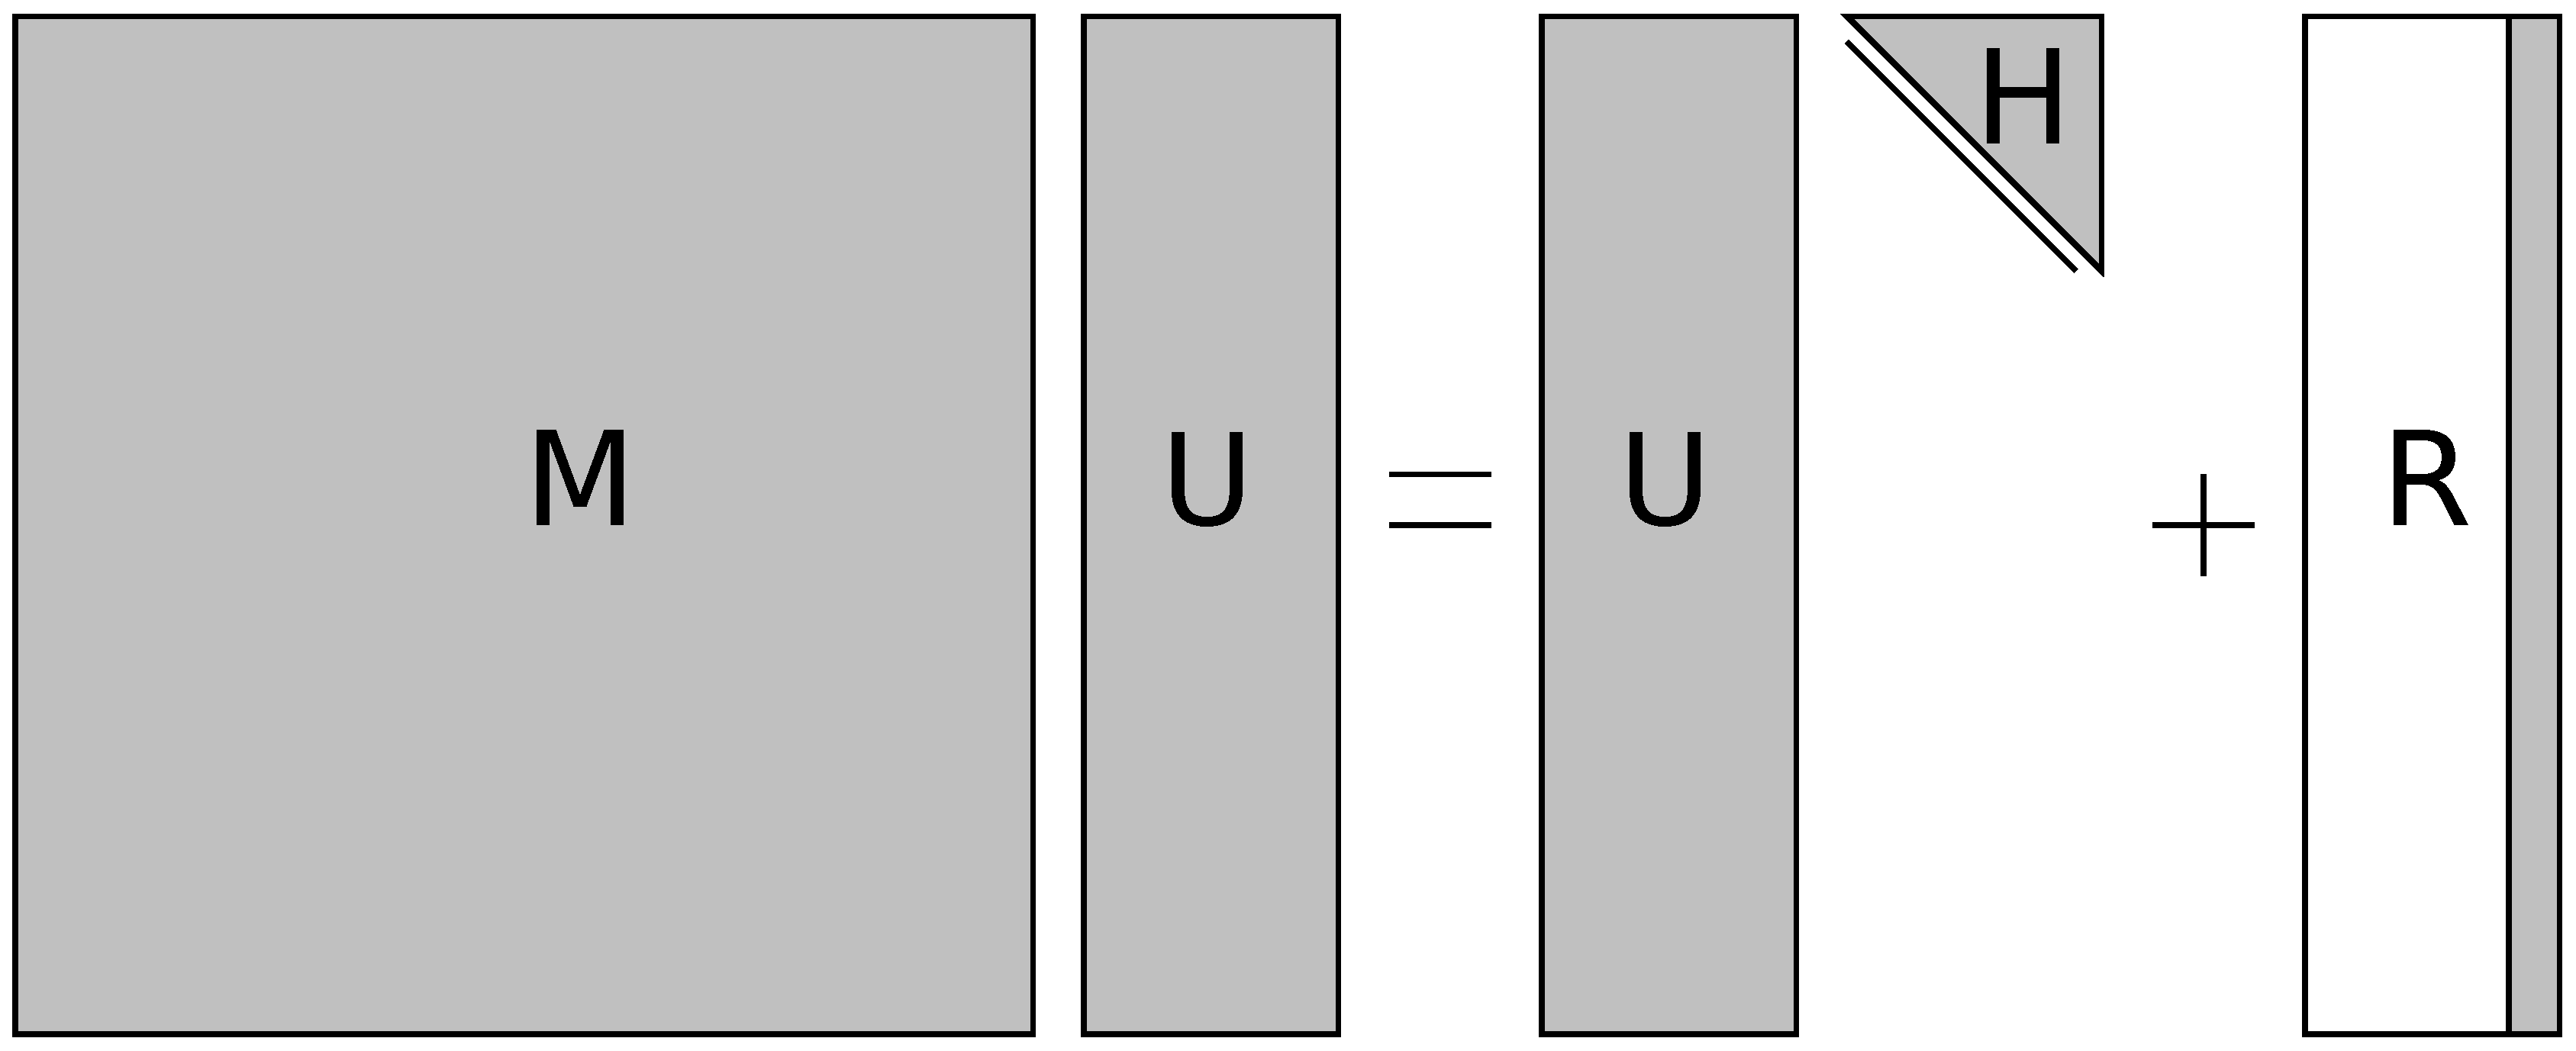
\includegraphics[width=.75\textwidth]{Arnoldi_structure}
      \caption{\emph{Arnoldi decomposition} -- Given a matrix $\mathbfcal{M} \in \mathbb{R}^{n \times n}$, construct an orthonormal set of vectors $\mathbfcal{V} \in \mathbb{R}^{n \times k}$ such that $\mathbfcal{H} \in \mathbb{R}^{k \times k}$ is an upper Hessenberg matrix and only the last column of the residual matrix $\mathbfcal{R} \in \mathbb{R}^{n \times k}$ is nonzero. Figure has been adapted from \cite{book:antoulas:2005}.}
      \label{fig: numerics -- arnoldi decomposition structure}
    \end{figure}

    \begin{figure}[b]
      \centering
      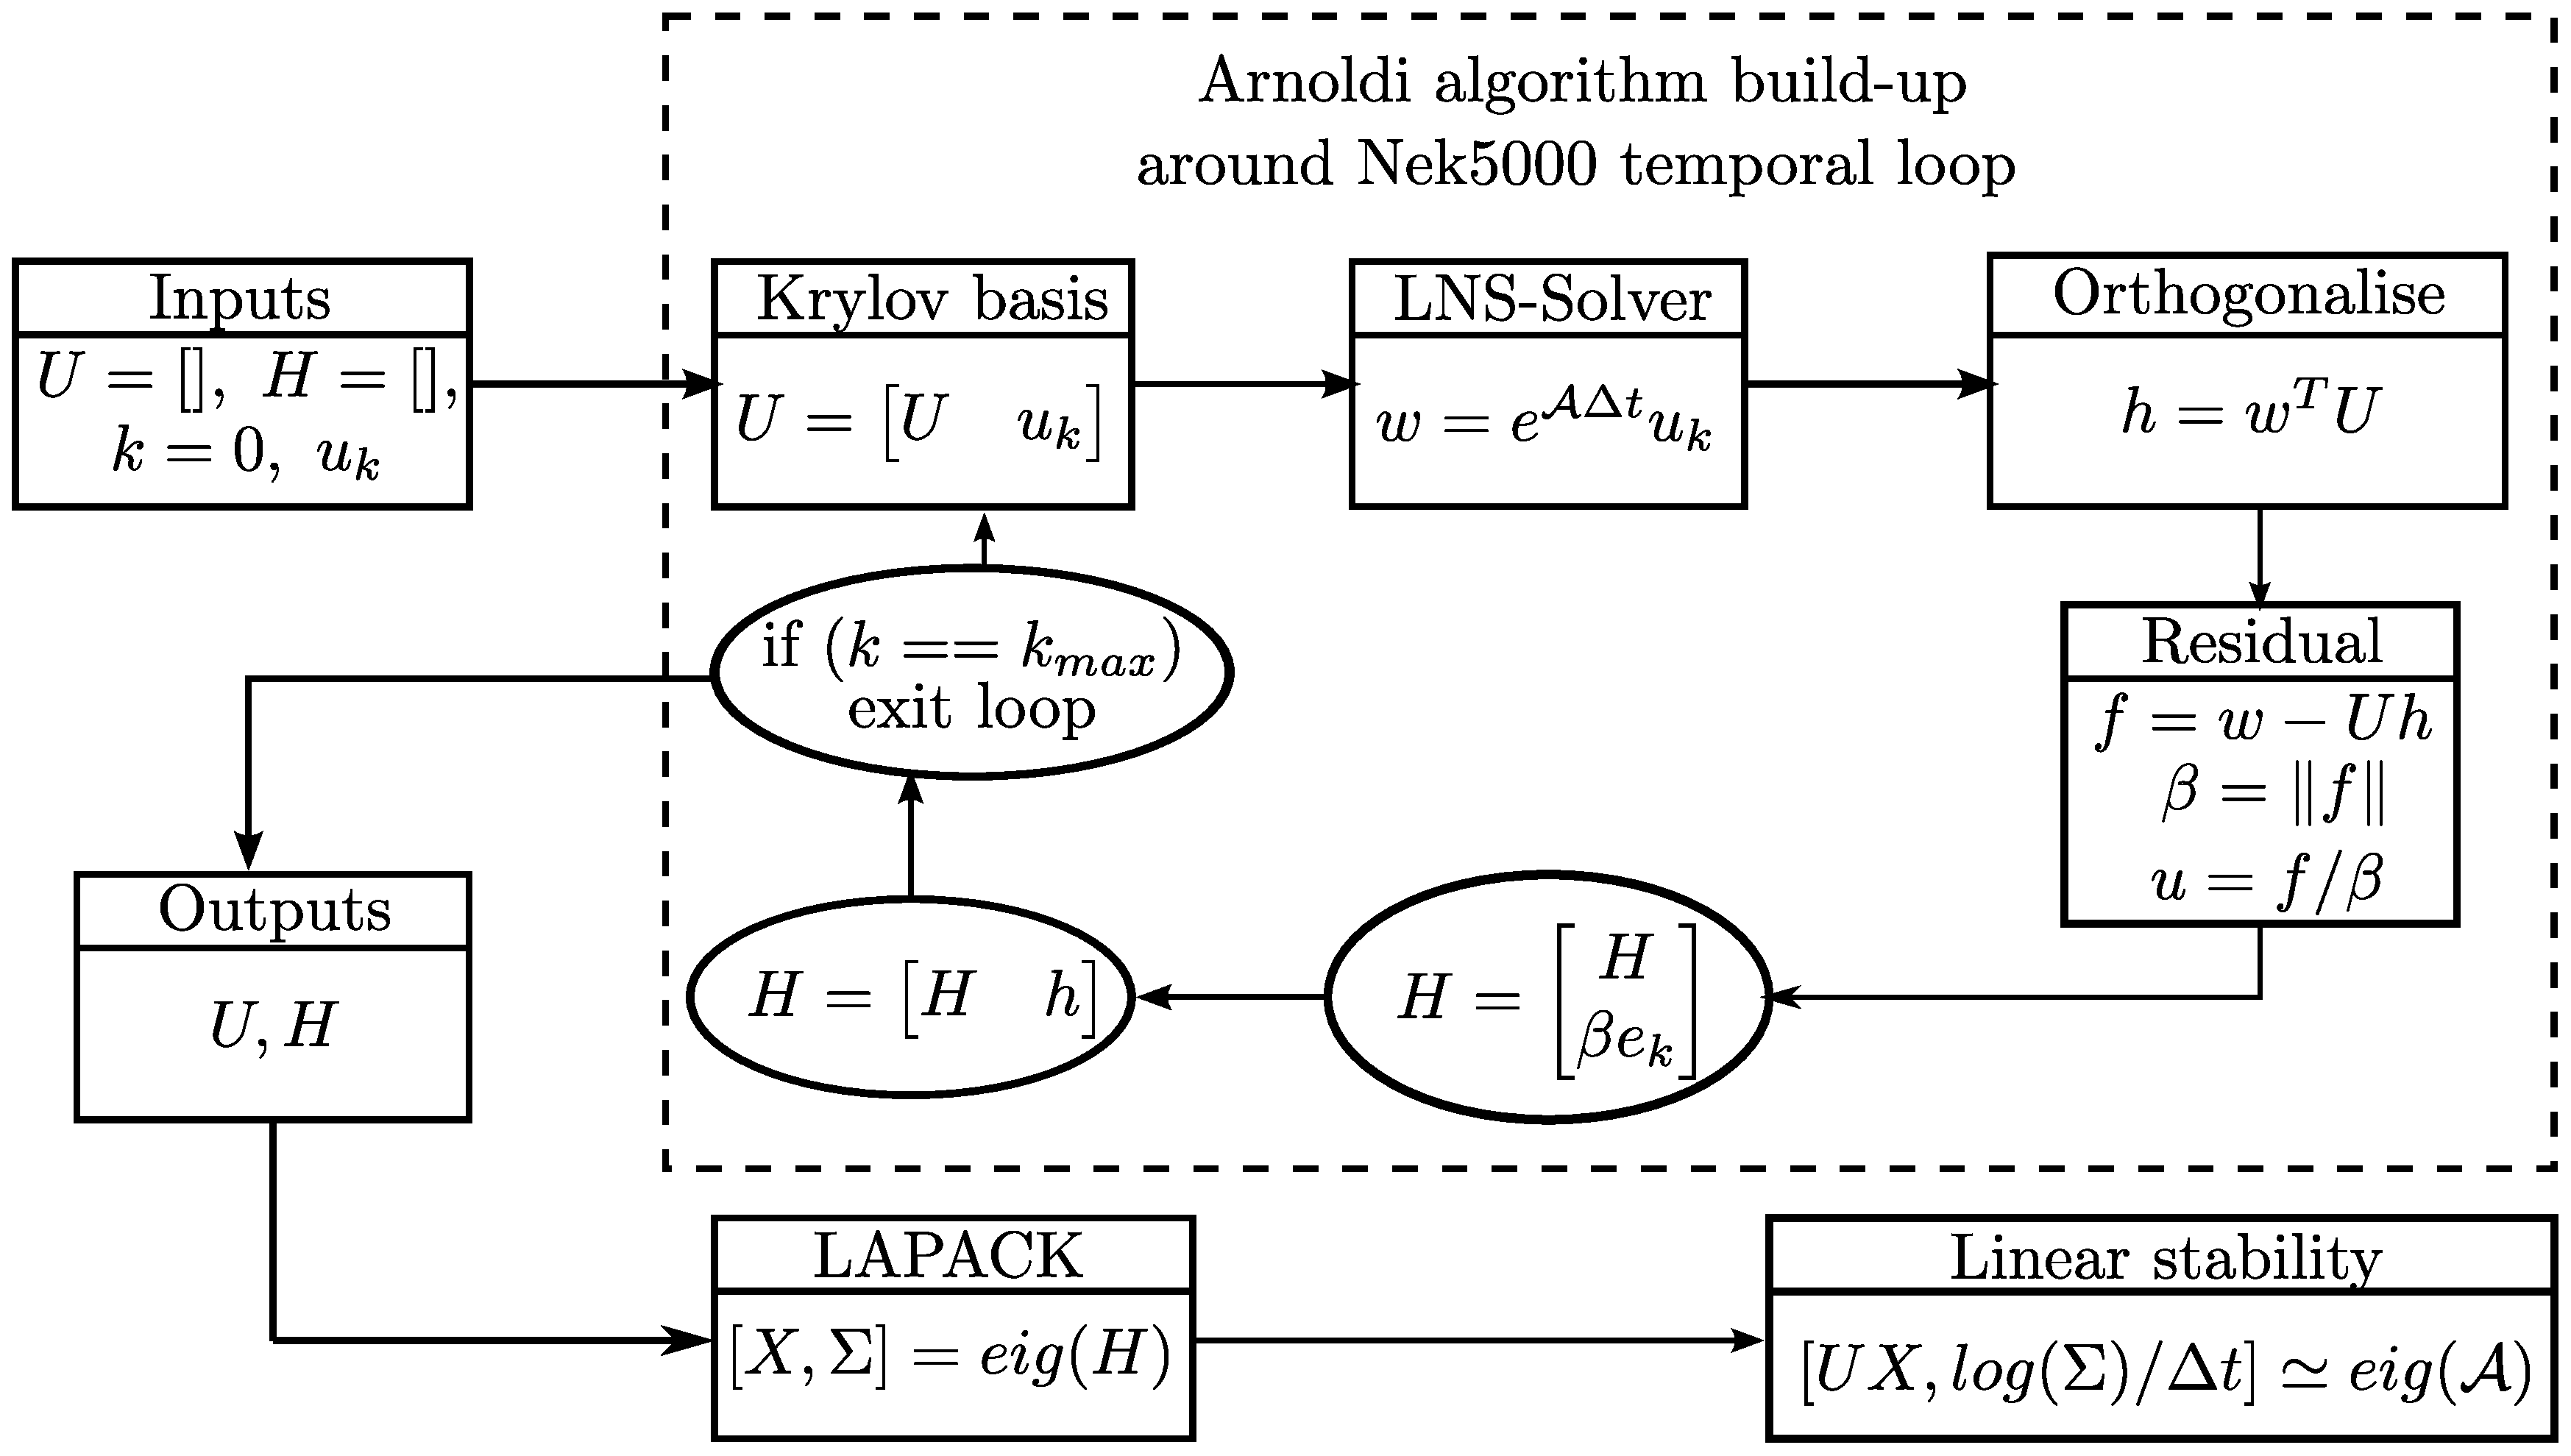
\includegraphics[width=.9\textwidth]{Arnoldi}
      \caption{Block-diagram representation of the basic $m$-step Arnoldi factorization. Note that, within a time-stepper framework, every matrix-vector product $\mathbfcal{M} \mathbf{v}_i$ is evaluated by marching in time the linearized system considered.}
      \label{fig: numerics -- arnoldi decomposition}
    \end{figure}

    %-----> Krylov-Schur decomposition.
    \subsubsection{Krylov-Schur decomposition}
    \label{subsubsec: numerics -- krylov-schur}

    Let us consider the $m$-step Arnoldi factorization
    \begin{equation}
      \mathbfcal{MV}_m = \mathbfcal{V}_m \mathbfcal{H}_m + \beta \mathbf{v}_{m+1} \mathbf{e}^T_m
      \label{eq: m-step Arnoldi}
    \end{equation}
    introduced in \textsection \ref{subsubsec: numerics -- arnoldi}. As discussed previously, the Ritz pair $\left( \mu_H, \mathbfcal{V}_m \mathbf{y} \right)$ of $\mathbfcal{H}_m$ provides a good approximation for the eigenpair $\left( \mu, \hat{\mathbf u} \right)$ of the matrix $\mathbfcal{M}$. One limitation of the Arnoldi decomposition is however that the dimension $m$ of the Krylov subspace necessary to converge the leading Ritz pairs is not known \emph{a priori}. It might hence be relatively large, thus potentially causing some numerical and/or practical problems (e.g.\ storage of Krylov basis $\mathbfcal{V}_m$, forward instability of the Gram-Schmidt process involved in the Arnoldi decomposition, etc). Two different approaches have been proposed to overcome these limitations: the \emph{Implicitly Restarted Arnoldi Method} introduced by Sorensen \cite{Sorensen_SIAM_1992} in 1992 and the \emph{Krylov-Schur decomposition} introduced by Stewart \cite{Stewart_SIAM_2001} in 2001. In the present work, the latter approach has been preferred because of its simplicity of implementation and its robustness.

    The Krylov-Schur method is based on the generalization of the m-step Arnoldi factorization~\eqref{eq: m-step Arnoldi} to a \emph{Krylov decomposition} of order $m$
    \begin{equation}
      \mathbfcal{MV}_m = \mathbfcal{V}_m \mathbfcal{B}_m + \mathbf{v}_{m+1} \mathbf{b}_{m+1}^T
      \label{eq: Krylov decomposition}
    \end{equation}
    for which the matrix $\mathbfcal{B}_m$ and the vector $\mathbf{b}_{m+1}$ have no restriction. The Arnoldi decomposition then appears as a special case of Krylov decomposition where $\mathbfcal{B}_m$ is restricted to be in upper Hessenberg form and $\mathbf{b}_{m+1} = \mathbf{e}_m$. Another special case is the \emph{Krylov-Schur} decomposition for which the matrix $\mathbfcal{B}_m$ is in real Schur form (i.e.\ quasi-triangular form with its eigenvalues in the $1 \times 1$ or $2 \times 2$ diagonal blocks). It has been shown by Stewart \cite{Stewart_SIAM_2001} that Krylov and Arnoldi decompositions are equivalent (i.e.\ they have the same Ritz approximations). Moreover, by means of orthogonal similarity transformations, any Krylov decomposition can be transformed into an equivalent Krylov-Schur decomposition.

    The core of the Krylov-Schur method is based on a two-steps procedure: (\emph{i}) an expansion step performed using a $m$-step Arnoldi factorization, and (\emph{ii}) a contraction step to a Krylov-Schur decomposition of order $p$ retaining only the most useful spectral information from the initial $m$-step Arnoldi decomposition. Given an initial unit-norm vector $\mathbf{v}_1$, a subroutine to compute the matrix-vector product $\mathbfcal{M} \mathbf{v}_i$, and the desired dimension $m$ of the Krylov subspace, the Krylov-Schur method can be summarized as follows:
    \begin{enumerate}
      \item Construct an initial Krylov decomposition of order $m$ using for instance the $m$-step Arnoldi factorization~\eqref{eq: m-step Arnoldi}.

      \item Check for the convergence of the Ritz eigenpairs. If a sufficient number has converged, then stop. Otherwise, proceed to step 3.

      \item Compute the real Schur decomposition $\mathbfcal{B}_m = \mathbfcal{Q} \mathbfcal{S}_m \mathbfcal{Q}^T$ such that the matrix $\mathbfcal{S}_m$ is in real Schur form and $\mathbfcal{Q}$ is the associated matrix of Schur vectors. It is assumed furthermore that the Ritz values on the diagonal blocks of $\mathbfcal{S}_m$ have been sorted such that the $p$ ''wanted'' Ritz values are in the upper-left corner of $\mathbfcal{S}_m$, while the $m-p$ ''unwanted'' ones are in the lower-right corner. At this point, we have the following re-ordered Krylov-Schur decomposition
      \begin{equation}
        \mathbfcal{M} \tilde{\mathbfcal{V}}_m =
        \tilde{\mathbfcal{V}}_m
        \begin{bmatrix}
         \mathbfcal{S}_{11} & \mathbfcal{S}_{12} \\
         {\mathbf 0}     & \mathbfcal{S}_{22}
       \end{bmatrix}
       + {\mathbf v}_{m+1}\begin{bmatrix}
                           {\mathbf b}_{1}^T & {\mathbf b}_{2}^T
                           \end{bmatrix}
        \label{eq: Krylov-Schur decomposition}
      \end{equation}
      with $\tilde{\mathbfcal{V}}_m = \mathbfcal{V}_m  \mathbfcal{Q}$ being the re-ordered Krylov basis, $\mathbfcal{S}_{11}$ the subset of the Schur matrix containing the $p$ ''wanted'' Ritz values, $\mathbfcal{S}_{22}$ the subset containing the $m-p$ ''unwanted'' ones, and $\begin{bmatrix} {\mathbf b}_1^T & {\mathbf b}_2^T \end{bmatrix} = {\mathbf b}^T \mathbfcal{Q}$.

      \item Truncate the Krylov-Schur decomposition~\eqref{eq: Krylov-Schur decomposition} of order $m$ to a Krylov decomposition of order $p$,
        \begin{equation}
          \mathbfcal{M}\tilde{\mathbfcal{V}}_p = \tilde{\mathbfcal{V}}_p \mathbfcal{S}_{11} + \tilde{\mathbf v}_{p+1}{\mathbf b}_1^T
        \end{equation}
      with $\tilde{\mathbfcal{V}}_p$ equal to the first $p$ columns of $\tilde{\mathbfcal{V}}_m$ and $\tilde{\mathbf v}_{p+1} = {\mathbf v}_{m+1}$.

      \item Extend again to a Krylov decomposition of order $m$ using a variation of the procedure used in the first step: the procedure is re-initialized with the starting vector ${\mathbf v}_{p+1}$ but all the vectors in $\tilde{\mathbfcal{V}}_p$ are taken into account in the orthogonalization step.

      \item Check the convergence of the Ritz values. If not enough Ritz values have converged, restart from step 3.

    \end{enumerate}
    This algorithm has two critical steps. The first one is the choice of the ''wanted'' Ritz values in the re-ordering of the Schur decomposition in step 2. Since we are only interested in the leading eigenvalues of the linearized Navier-Stokes operator, all the Ritz pairs being classified as ''wanted'' must satisfy $\left| \mu_w \right| \ge 1 - \delta$ (with $\delta = 0.05 - 0.1$ usually). Regarding the criterion assessing the convergence of a given Ritz pair, starting from the Krylov decomposition~\eqref{eq: m-step Arnoldi}, one can write
    \begin{equation}
      \| \mathbfcal{M} \mathbfcal{V}_m \mathbf{y} - \mathbfcal{V}_m \mathbfcal{B}_m \mathbf{y} \| = \| \mathbfcal{M} \mathbfcal{V}_m \mathbf{y} - \mu_{\mathbf B} \mathbfcal{V}_m \mathbf{y} \| = \left| \beta \mathbf{e}_m^T \mathbf{y} \right|
      \label{eq: Krylov convergence}
    \end{equation}
    with $(\mu_{\mathbf B},\mathbf{y})$ a given eigenpair of the matrix $\mathbfcal{B}_m$. If the right hand side $\left| \beta {\mathbf e}_{m}^T{\mathbf y} \right|$ is smaller than a given tolerance, then the Ritz pair $(\mu_{\mathbf B}, \mathbfcal{V}_m {\mathbf y})$ provides a good approximation to the eigenpair $(\mu, \hat{\mathbf u})$ of the original matrix $\mathbfcal{M}$. A Ritz value is generally considered as being converged if the associated residual $\left| \beta {\mathbf e}_{m}^T{\mathbf y} \right| \le 10^{-6}$.

    %-----> Comparisons.
    \subsubsection{Comparison of the two approaches}
    \label{subsubsec: numerics -- comparison arnoldi krylov-schur}

    Following the comparison of the fixed points solvers in \textsection \ref{subsubsec: numerics -- fixed points comparison}, let us now compare the efficiency of the time-stepper Krylov-Schur decomposition over the Arnoldi one when computing the leading eigenvalues and eigenmodes of the linearized Navier-Stokes operator for the shear-driven cavity flow at $Re=4150$. For that purpose, the eigenspectrum obtained using the Arnoldi decomposition with a Krylov subspace of dimension $k_{\mathrm{dim}}=256$ will serve as our reference point. For the sake of comparison, three Krylov subspaces of various dimensions, namely $k_{\mathrm{dim}}=$192, 128 and 64 have been considered for the Krylov-Schur decomposition. In all cases, twelve eigenvalues were required to have converged with a residual $\epsilon \le 10^{-6}$ before the computation could stop. Finally, the sampling period has been set to $T = 0.2$ non-dimensional time units so that the exponential propagator (whose action is approximated by time-marching the linearized Navier-Stokes equation) is given by $\mathbfcal{M} = \exp \left( 0.2 \mathbfcal{A} \right)$, with $\mathbfcal{A}$ being the linearized Navier-Stokes operator.

    Left panel of figure \ref{fig: numerics -- linear stability eigenpairs} depicts the eigenspectra obtained using the Arnoldi decomposition with a Krylov subspace dimension $k_{\mathrm{dim}}=256$ and Krylov-Schur decomposition with $k_{\mathrm{dim}}=128$ and $k_{\mathrm{dim}}=64$, while its right panel shows the real part of the streamwise velocity component of some of the leading eigenmodes for the sake of completeness. These plots highlight the existence of two families of modes: (\textit{i}) high-frequency shear layer modes (also known as \emph{R\"ossiter} modes), and (\textit{ii}) low-frequency inner-cavity modes similar to the ones existing in lid-driven cavities. A detailed description of the physical mechanisms underlying these instabilities is beyond the scope of the present work. Interested readers are referred to \cite{BLLFD2011} regarding the shear layer instability modes and \cite{FALP2007,FPLFB2009} for the inner-cavity instabilities.

    Table \ref{tab: numerics -- linear stability comparison} reports the growth rate $\sigma$ and circular frequency $\omega$ of the leading eigenvalue for all of the cases considered. Even with a Krylov subspace four times smaller than the reference one, it can be seen that the leading eigenvalue's growth rate computed by the Krylov-Schur decomposition differs by less than 0.02\% compared to our reference solution while the circular frequency is left unchanged at least until the fifth digit. The major difference between $k_{\text{dim}} = 256$ and $k_{\text{dim}}=64$ is the accuracy of the eigenvalues belonging to the branches of inner-cavity modes, see figure \ref{fig: numerics -- linear stability eigenpairs}. These modes however turn out to be of limited interest in the dynamics of the flow.

    Finally, the last row of table \ref{tab: numerics -- linear stability comparison} reports the total number of calls to the linearized Navier-Stokes solver necessary to converge the required twelve eigenvalues. Compared to our reference case (i.e.\ $k_{\text{dim}}=256$), the total number of matrix-vector multiplications is inversely proportional to the reduction factor of the dimension of the Krylov subspace considered. Despite this increase of the number of matrix-vector multiplications, Krylov-Schur decomposition with a moderate subspace dimension (e.g.\ $k_{\text{dim}}=64$ or 128) has nonetheless two major benefits compared to the classical Arnoldi decomposition:
    \begin{itemize}
      \item \emph{Reduced memory footprint}: having a smaller Krylov subspace implies that fewer Krylov vectors need to be stored. This may be of crucial importance if one consider very large-scale eigenvalue problems such as the ones appearing in fluid dynamics (see \cite{jfm:ilak:2012, jfm:loiseau:2014, pof:citro:2015, jfm:bucci:2018} for illustrations) which need to be solved on high-performance computers.

      \item \emph{Partially reduced computation complexity}: although table \ref{tab: numerics -- linear stability comparison} underlines that a larger number of calls to the linearized time-stepper code is required as we decrease the size of the Krylov subspace, one must not overlook that Arnoldi decomposition necessitates modified Gram-Schmidt orthogonalization of the Krylov sequence to iteratively construct the upper Hessenberg matrix. For an $n \times k$ matrix (where $n$ is the number of degrees of freedom and $k$ the dimension of the Krylov subspace), the computational complexity of this step scales as $nk^2$. As a consequence, decreasing the size of the Krylov subspace by a factor 4 reduces the computational cost of the modified Gram-Schmidt orthogonalization by a factor 16. Such a reduction becomes particularly attractive if ones needs a very large Krylov subspace to converge the leading eigenvalues when using the classical Arnoldi decomposition.
    \end{itemize}
    Finally, although Krylov-Schur decomposition does have some benefits compared to the classical Arnoldi iteration, it must not be forgotten that the overall computational time is dictated by the linearized time-stepper solver used to evaluate the application of the exponential propagator $\mathbfcal{M}$ onto a given vector. Consequently, efficient and scalable temporal integrators are key enablers for very large-scale eigenvalue analysis arising from the discretization of partial differential equations. Discussion on efficient and scalable temporal and/or spatial discretization is however beyond the scope of this contribution.

    \begin{figure}
      \centering
      \includegraphics[scale=1]{S3_eigenpairs}
      \caption{Eigenspectrum and leading eigenmodes (streamwise velocity field) for the shear-driven cavity flow at $Re=4150$. Blue circles ({\color{blue} $\boldsymbol{\circ}$}) depict the eigenvalues obtained using the Arnoldi decomposition (see \textsection \ref{subsubsec: numerics -- arnoldi}) with a Krylov subspace of dimension $k_{\mathrm{dim}} = 256$ while orange squares ({\color{orange} $\square$}) and green crosses ({\color{green} $\times$}) depict the eigenvalues obtained using the Krylov-Schur decomposition (see \textsection \ref{subsubsec: numerics -- krylov-schur}) with a Krylov subspace of dimension $k_{\mathrm{dim}}=128$ and $k_{\mathrm{dim}} = 64$, respectively. In both cases, the computation stopped once the twelve eigenvalues have been converged down to $\epsilon = 10^{-6}$.}
      \label{fig: numerics -- linear stability eigenpairs}
    \end{figure}

    \begin{table}
      \caption{Growth rate $\sigma$ and circular frequency $\omega$ of the leading eigenvalue computed for different dimensions of the Krylov subspace. Note that only the largest Krylov subspace (i.e.\ $k_{\mathrm{dim}}=256$) uses the basic Arnoldi decomposition. All other computations have been performed with Krylov-Schur. The total number of calls to the linearized Navier-Stokes solver (i.e.\ the number of Jacobian matrix-vector multiplications) is also reported for each case.}
      \label{tab: numerics -- linear stability comparison}
      \begin{tabular}{p{2cm}p{2.5cm}p{2.5cm}p{2.5cm}p{2.5cm}}
      \hline\noalign{\smallskip}
       & $k_{\mathrm{dim}} = 256$ & $k_{\mathrm{dim}} = 192$ & $k_{\mathrm{dim}} = 128$ & $k_{\mathrm{dim}} = 64$  \\
      \noalign{\smallskip}\svhline\noalign{\smallskip}
      $\sigma$  & $4.56757 \cdot 10^{-3}$ & $4.56757 \cdot 10^{-3}$ & $4.56757 \cdot 10^{-3}$ & $4.56673 \cdot 10^{-3}$\\
      $\omega$ & $\pm 7.4938$ & $\pm 7.4938$ & $\pm 7.4938$ & $\pm 7.4938$\\
      Matrix-vector multiplications & 256 & 384 & 512 & 832\\
      \noalign{\smallskip}\hline\noalign{\smallskip}
      \end{tabular}
    \end{table}
  %%%%%%%%%%%%%%%%%%%%%%%%%%%%%%%%%%%%%%%%%%%%%%%%
  %%%%%                                      %%%%%
  %%%%%     NON-MODAL STABILITY ANALYSIS     %%%%%
  %%%%%                                      %%%%%
  %%%%%%%%%%%%%%%%%%%%%%%%%%%%%%%%%%%%%%%%%%%%%%%%

  \subsection{Non-modal stability and singular value decomposition}

  Given the linear time-invariant dynamical system
  \begin{equation}
    \dot{\mathbf{x}} = \mathbfcal{A} \mathbf{x} + \mathbf{f},
    \notag
  \end{equation}
  it has been shown in \textsection \ref{subsec: theory -- linear stability} that, for $\mathbf{f} = \mathbf{0}$ (i.e.\ no external forcing), the asymptotic fate of a random initial condition $\mathbf{x}_0$ is dictated by the eigenpairs of the Jacobian matrix $\mathbfcal{A}$. On the other hand, as shown in \textsection \ref{subsec: theory -- non-modal stability}, its short-term dynamics are governed by the singular triplets of the exponential propagator $\mathbfcal{M} = \exp \left( \mathbfcal{A} T \right)$, where $T$ is the time horizon considered. Conversely, the asymptotic response of the (stable) system to an external forcing $\mathbf{f}$ is governed by the singular triplets of the so-called resolvent operator $\mathbfcal{R} = \left( i\omega \mathbfcal{I} - \mathbfcal{A} \right)^{-1}$, where $\omega$ is the forcing frequency. The rest of this section is devoted to the presentation of two different time-stepper algorithms for the computation of the leading singular values and singular vectors of the exponential propagator $\mathbfcal{M}$ or the resolvent operator $\mathbfcal{R}$.

  %-----> Optimization point of view.
  \subsubsection{An optimization approach}

  It has been shown in \textsection \ref{subsec: theory -- non-modal stability} that optimal perturbation analysis could be formulated as an optimization problem given by
  \begin{equation}
      \begin{aligned}
        \maximize \limits_{\mathbf{x}_0} & \mathcal{J} \left( \mathbf{x}_0 \right) = \| \mathbf{x}(T) \|_2^2\\
        \subjecto & \dot{\mathbf{x}} - \mathbfcal{A}\mathbf{x} = 0 \\
        ~ & \| \mathbf{x}_0 \|_2^2 - 1 = 0,
      \end{aligned}
      \label{eq: numerics -- optimal perturbation constrained maximization}
  \end{equation}
  where $\mathcal{J}(\mathbf{x}_{0})$ is known as the \emph{objective function}. Similarly, the optimal forcing problem can be formulated as
  \begin{equation}
      \begin{aligned}
        \maximize \limits_{\hat{\mathbf{f}}} & \mathcal{J} \left(    \hat{\mathbf{f}} \right) = \| \hat{\mathbf{x}}(\omega) \|_2^2\\
        \subjecto & \left( i \omega \mathbfcal{I} - \mathbfcal{A} \right) \hat{\mathbf{x}} = \hat{\mathbf{f}} \\
        ~ & \| \hat{\mathbf{f}} \|_2^2 - 1 = 0,
      \end{aligned}
      \label{eq: numerics -- optimal forcing constrained maximization}
  \end{equation}
  Though these optimization problems are non-convex, solutions to both of them can be obtained by means of standard gradient-based optimization algorithms. One of the most famous such algorithms is the \emph{conjugate gradient} method originally introduced by \cite{book:hestenes:1952}, see \cite{book:saad:2003} and \cite{book:golub:2012} for more recent presentations. In this work we will however introduce the reader to the \emph{rotation update} technique, a modification of the classical steepest ascent method based on geometric considerations. Figure \ref{fig: numerics -- rotation update gradient} provides a schematic description of this algorithm. This approach has been used by \cite{jfm:foures:2013, jfm:foures:2014} and \cite{fdr:farano:2016} in the context of \emph{p-norms} optimization in fluid dynamics.

  Both Eq.\ \eqref{eq: numerics -- optimal perturbation constrained maximization} and Eq.\ \eqref{eq: numerics -- optimal forcing constrained maximization} are constrained maximization problems. As shown in \textsection \ref{subsec: theory -- non-modal stability}, introducing Lagrange multipliers allows us to transform these constrained problems into equivalent unconstrained ones. For the optimal perturbation analysis, the unconstrained maximization problem thus reads
  \begin{equation}
    \maximize \limits_{\mathbf{x}, \mathbf{v}, \mu} \mathcal{L} \left( \mathbf{x}, \mathbf{v}, \mu \right),
    \label{eq: numerics -- unconstrained maximization}
  \end{equation}
  where
  \begin{equation}
    \mathcal{L} \left( \mathbf{x}, \mathbf{v}, \mu \right) = \mathcal{J}\left( \mathbf{x}_0 \right) + \int_{0}^T \mathbf{v}^T \left( \dot{\mathbf{x}} - \mathbfcal{A}\mathbf{x} \right) \mathrm{d}t + \mu \left( \| \mathbf{x}_0 \|_2^2 - 1 \right)
    \label{eq: numerics -- augmented Lagrangian}
  \end{equation}
  is known as the \emph{augmented Lagrangian} function. The additional optimization variables $\mathbf{v}$ and $\mu$ appearing in the definition of the augmented Lagrangian $\mathcal{L}$ are the \emph{Lagrange multipliers}. The gradient of the augmented Lagrange functional $\mathcal{L}$ with respect to the initial condition $\mathbf{x}_0$ reads
  \begin{equation}
    \displaystyle \frac{\partial \mathcal{L}}{\partial \mathbf{x}_0} = 2\mu\mathbf{x}_0 - \mathbf{v}_0.
  \end{equation}
  This expression explicitly depends on the Lagrange multiplier $\mu$ whose value is unfortunately unknown. One can however write down a mathematical expression of this gradient orthogonalized with respect to the input $\mathbf{x}_0$
  \begin{equation}
      \frac{\partial \mathcal{L}}{\partial {\bf x}}^{\perp} = \frac{\partial \mathcal{L}}{\partial {\bf x}} - \frac{\langle \frac{\partial \mathcal{L}}{\partial {\bf x}},{\bf x} \rangle}{\langle {\bf x},{\bf x} \rangle}{\bf x}
  \end{equation}
  where $\langle \cdot,\cdot \rangle$ stands for the inner product. Note moreover that we dropped the subscript 0 for the sake of simplicity. It can now be expressed as
  \begin{equation}
      \frac{\partial \mathcal{L}}{\partial {\bf x}}^{\perp} = ({\bf v} - 2\mu {\bf x}) - \frac{\langle ({\bf v} - 2\mu {\bf x}) , {\bf x} \rangle}{\langle {\bf x},{\bf x} \rangle}{\bf x}
  \end{equation}
  After simplifications, the orthogonalized gradient finally reads
  \begin{equation}
    \frac{\partial \mathcal{L}}{\partial {\bf x}}^{\perp} = \mathbf{v} - \frac{\langle \mathbf{v},{\bf x} \rangle}{\langle {\bf x},{\bf x} \rangle}{\bf x}
    \label{eq: orthogonalised gradient}
  \end{equation}
  This expression now solely depends on the direct variable ${\bf x}$ and the adjoint one ${\bf v}$, while the dependence on the unknown Lagrange multiplier $\mu$ has been completely removed from the optimization problem. Normalizing this new gradient such that
  \begin{equation}
    {\bf G}^n = \sqrt{\frac{\| \mathbf{x}_0 \|_2^2}{\langle \frac{\partial \mathcal{L}}{\partial {\bf x}}^{\perp},\frac{\partial \mathcal{L}}{\partial {\bf x}}^{\perp} \rangle}} \frac{\partial \mathcal{L}}{\partial {\bf x}}^{\perp}
  \end{equation}
  now allows us to look for the update ${\bf x}^{n+1}$ as a simple linear combination of ${\bf x}^n$ and ${\bf G}^n$ given by
  \begin{equation}
    {\bf x}^{n+1} = \cos(\alpha) {\bf x}^n + \sin(\alpha) {\bf G}^n
  \end{equation}
  Since ${\bf x}^n$ and ${\bf G}^n$ form an orthonormal set of vectors, the update ${\bf x}^{n+1}$ fulfills, directly by construction, the constraint on the amplitude of the initial perturbation. No quadratic equation in $\mu$, as in the case of steepest ascent method, need to be solved anymore at each iteration of the optimization loop. To ensure the convergence of the method to the maxima of the augmented functional $\mathcal{L}$, a check needs however to be put on the value of the angle $\alpha$ used for the update of the solution. Every calculations presented in this work uses $\alpha=0.5$ as the initial value. If the value of the cost function $\mathcal{J}$ computed at the $(n+1)$\textsuperscript{th} iteration is smaller than the value of $\mathcal{J}$ at the previous one, then the update ${\bf x}^{n+1}$ is re-updated with a different value of $\alpha$, typically $\alpha = \alpha/2$ until the new value of $\mathcal{J}$ is larger than the previous one.

  \begin{figure}
    \centering
    \includegraphics[width=\textwidth]{S3_rotation_update_gradient}
    \caption{Schematic representation of the \emph{rotation update} method. (a) Compute the gradient $\nicefrac{\partial \mathcal{L}}{\partial \mathbf{x}}$ of the augmented Lagrange functional. (b) Orthogonalise the gradient with respect to $\mathbf{x}^n(0)$. (c) Compute $\mathcal{G}^n$, i.e.\ the orthogonalized gradient normalized such that its energy is $E_0$. (d) Update $\mathbf{x}^{n+1}(0)$ using a linear combination $\mathbf{x}^n(0)$ and of the orthonormalized gradient $\mathbf{G}^n$.}
    \label{fig: numerics -- rotation update gradient}
  \end{figure}

  %-----> Formulation as an SVD problem.
  \subsubsection{Singular value decomposition}

  Formulating the optimal perturbation analysis as a maximization problem yields a non-convex optimization problem. As a consequence, one cannot rule out the possibility that gradient-based algorithms get stuck on a local maximum. Hopefully, it has been shown in \textsection \ref{subsec: theory -- non-modal stability} that the same problem could be formulated as a singular value decomposition of either the exponential propagator $\mathbfcal{M} = \exp \left( \mathbfcal{A} T \right)$ or the resolvent one $\mathbfcal{R} = \left( i \omega \mathbfcal{I} - \mathbfcal{A} \right)^{-1}$, depending on the problem considered.

  Let us consider once more the optimal perturbation problem for the sake of simplicity, although the derivation to be given naturally extend to the case to the resolvent. Given the singular value decomposition of the exponential propagator
  \begin{equation}
    \mathbfcal{M} \triangleq \exp \left( \mathbfcal{A} T \right) = \mathbfcal{U} \boldsymbol{\Upsigma} \mathbfcal{V}^H,
    \notag
  \end{equation}
  the optimal perturbation at $t=0$ is given by the right singular vector $\mathbf{v}_1$, i.e.\ the first column of $\mathbfcal{V}$, while the associated response at time $t=T$ is given by the rescaled left singular vector $\sigma_1 \mathbf{u}_1$, where $\sigma_1$ is the associated singular value characterizing the amplification of the perturbation. Computing directly the singular values and singular vectors of $\mathbfcal{M}$ is a challenging task for very large scale problems. Hopefully, introducing the adjoint exponential propagator $\mathbfcal{M}^{\dagger} = \exp \left( \mathbfcal{A}^{\dagger} T \right)$, readers can easily be convinced that our problem can be recast as the following equivalent eigenvalue problems
  \begin{equation}
    \mathbfcal{M}^{\dagger} \mathbfcal{M} \mathbf{v} = \sigma^2 \mathbf{v} \quad \text{and} \quad \mathbfcal{M} \mathbfcal{M}^{\dagger} \mathbf{u} = \sigma^2 \mathbf{u}.
    \label{eq: numerics -- singular value decomposition as eigenvalue problem}
  \end{equation}
  From a practical point of view, evaluating the action of the matrix $\mathbfcal{M}^{\dagger} \mathbfcal{M}$ onto a vector $\mathbf{x}$ can be computed in a two-step procedure:
  \begin{enumerate}
    \item Integrate forward in time the original system, $\mathbf{x}(T) = \exp \left( \mathbfcal{A} T \right) \mathbf{x}$.
    \item Integrate backward in time the adjoint problem using the output of the previous step as the initial condition, i.e.\ evaluating $\exp \left( \mathbfcal{A}^{\dagger} T \right) \mathbf{x}(T)$.
  \end{enumerate}
  Provided an adjoint time-stepper code is available, one can thus readily solve the optimal perturbation problem using the eigenvalue solvers described in \textsection \ref{subsubsec: numerics -- arnoldi} or \textsection \ref{subsubsec: numerics -- krylov-schur}. Moreover, given that $\mathbfcal{M}^{\dagger} \mathbfcal{M}$ is a symmetric positive-definite matrix, the upper Hessenberg matrix in the Arnoldi iteration can be replaced by a tri-diagonal matrix, hence resulting in the so-called \emph{Lanczos} iteration \cite{L1950}. Note finally that, when applied to the resolvent operator $\mathbfcal{R}$, the matrix-vector product $\mathbfcal{R}(\omega) \hat{\mathbf{f}}$ can be evaluated as follows:
  \begin{enumerate}
    \item Integrate forward in time the system $\dot{\mathbf{x}} = \mathbfcal{A} \mathbf{x} + \mathbf{f}(\omega)$.
    \item Perform a discrete Fourier transform of the asymptotic response to obtain $\hat{\mathbf{u}}(\omega)$.
  \end{enumerate}
  The same procedure applies for the action of $\mathbfcal{R}^{\dagger}(\omega)$ where one now needs to integrate backward in time the adjoint system using $\hat{\mathbf{u}}(\omega)$ as the external forcing. For more details about the computation of the optimal forcing using a time-stepper approach, readers are referred to \cite{jfm:monokrousos:2010}.

  %-----> Illustration
  \subsubsection{Illustration}

  As for modal stability (see \textsection \ref{subsubsec: numerics -- comparison arnoldi krylov-schur}), let us illustrate non-modal stability on the shear-driven cavity flow. For that purpose, the Reynolds number is set to $Re=4100$, i.e.\ slightly below the critical Reynolds number for the onset of linear instability. Only the optimal perturbation analysis (time-domain) will be presented for the sake of simplicity. For more details about the resolvent analysis (frequency domain), readers are referred to \cite{jfm:monokrousos:2010, phd:bucci:2017}. Figure \ref{fig: numerics -- illustration optimal perturbation analysis} depicts the evolution in time of the optimal perturbation's kinetic energy. It can be seen that, although linear stability analysis predicts that the flow is stable, perturbations can be amplified by 4 to 5 orders of magnitude solely through non-modal effects. Once the perturbation has reached its maximum transient amplification at $t=2$, its fate is eventually dictated by the least stable eigenvalue of the Jacobian matrix. Note that in the present case, the Reynolds number considered being slightly below that for the onset of instability, the eventual decay rate of the perturbation is relatively small. The perturbation nonetheless eventually disappears at $t \to +\infty$. Figure \ref{fig: numerics -- illustration optimal perturbation analysis} also clearly illustrates the different spatial support of the optimal initial perturbation (left panel) and the associated optimal response at $t=2$ (right panel). These different spatial supports result from the strong convective effects, which are related mathematically to the degree of non-normality of the Jacobian matrix. Similar observation holds true regarding the optimal forcing and optimal response when performing a resolvent analysis. Analysis of these transient (non-normal) effects may be of crucial importance when studying subcritical transition or for control purposes.

  Let us finally conclude this section by presenting the pros and cons of the SVD and optimization approaches. As discussed earlier, formulating the optimal perturbation and optimal forcing analyses in an optimization framework results in a non-convex optimization problem typically solved using gradient-based algorithms. Consequently, one cannot rule out the possibility that the solution returned by the optimization procedure actually corresponds to a local maxima of the problem at hand. On the other hand, formulating these two problems as singular value decompositions of the appropriate operator ensure that the solution obtained is indeed the optimal one by virtue of the Eckart-Young theorem. Moreover, singular value decomposition allows us to compute in one go not only the optimal perturbation but also the sub-optimal ones, something hardly possible within a classic optimization framework. Nonetheless, the optimization formulation offers much more flexibility than simply computing the optimal perturbation in the $\ell_2$ sense. Indeed, one can choose the objective function $\mathcal{J}(\mathbf{x})$ and the associated constraints according to the specific problem he/she aims to solve, see for instance \cite{jfm:foures:2013, jfm:foures:2014, fdr:farano:2016} for optimization based on the $\ell_1$ norm of the perturabtion.

  \begin{figure}
    \centering
    \includegraphics[scale=1]{S3_optimal_perturbation_analysis}
    \caption{Time-evolution of the optimal perturbation's kinetic energy for the shear-driven cavity flow at $Re=4100$, i.e.\ below the critical Reynolds number for the onset of linear instability. The lower panels depict the streamwise velocity of the initial optimal perturbation (left) and associated optimal response (right) at $T=2$.}
    \label{fig: numerics -- illustration optimal perturbation analysis}
  \end{figure}
  %
  % The energy amplification is driven by the non-normal features of the Jacobian matrix $\mathbfcal{A}$. Nevertheless, since the case in figure \ref{fig: numerics -- illustration optimal perturbation analysis} is close to the instability threshold the kinetic energy of the perturbation decay slowly to zero as expected by the global stability analysis.
